\section[Standard Model]{Standard Model}

\begin{frame}{Sub-atomic World}
\begin{center}
Particle Physics is the study of the properties of the fundamental building blocks of the universe and the interactions between them.
\\
\vspace{1em}
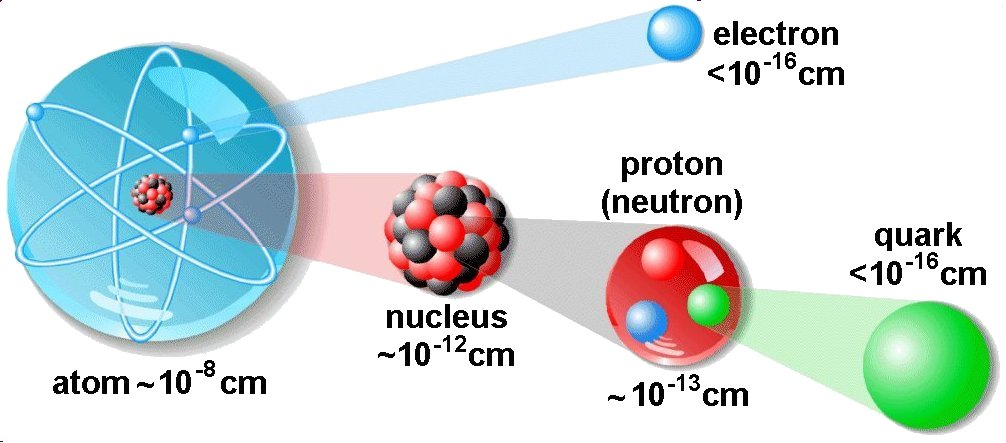
\includegraphics[width=0.99\textwidth]{images/subatomic_world.jpg}
\end{center}
\end{frame}


%\begin{frame}{Force}
%\begin{center}
%Force can be explained as the exchange of force carriers between particles.
%\\
%\vspace{1em}
%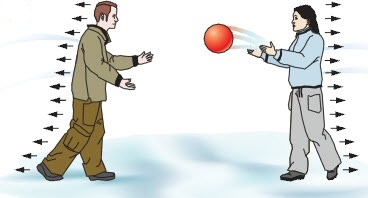
\includegraphics[width=0.69\textwidth]{images/force_exchange.jpg}
%\end{center}
%\end{frame}



\begin{frame}{The Four Fundamental Forces}
\begin{center}
There are four fundamental forces that we know of.
\\
\vspace{1em}
%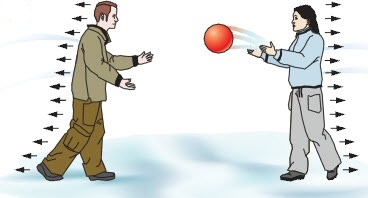
\includegraphics[width=0.69\textwidth]{images/force_exchange.jpg}
\begin{tabular}{ c c c c }
Force  & Boson    & Charge & Mass \\ \hline
Gravitational & graviton(G) & 0 & ? \\
Electromagnetic & photon($\gamma$) & 0 & 0 \\

\multirow{2}{*}{Weak} & W boson($W^{\pm}$) & $\pm$1 & 81 GeV \\
                      & Z boson(Z) & 0 & 92GeV \\

Strong & gluon(g) & 0      & 0 \\
\end{tabular}
\end{center}
\end{frame}




\begin{frame}{The Standard Model}
\begin{center}
The Standard Model is the compilation of over 100 years of scientific discoveries and is in excellent agreements with a wide range of experimental observations.
\\
\vspace{1em}
%\begin{columns}
 % \begin{column}{0.5\textwidth}
    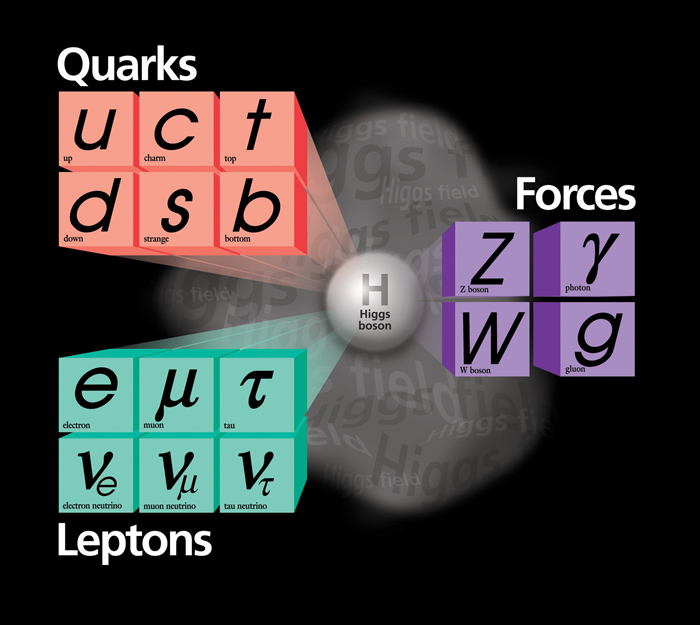
\includegraphics[width=0.49\textwidth]{images/standard_model_particles.jpg}
  %\end{column}
  %\begin{column}{0.5\textwidth}
  %\end{column}
\end{center}
\end{frame}

\begin{frame}{Particle Discoveries}
  \begin{center}
    \footnotesize
\begin{tabular}{ | c | c |}
  \hline
  Year & Discovery \\ \hline \hline
  1897 & e discovery, by J.J. Thompson (cathode ray tube, UK)\\ \hline
  1919 & proton, Ernest Rutherford (UK)\\ \hline
  1930 & neutron, James Chadwick (UK)\\ \hline
  1936 & m, Carl D. Anderson at Caltech\\ \hline
  1947 & strange quark(K+=usbar, K-=subar)\\ \hline
  1956 & $\nu_e$ discovery (nuclear reactor)\\ \hline
  1962 & $\nu_{\mu}$ discovery at BNL\\ \hline
  1968 & u and d quark (quark model)\\ \hline
  1974 & c quark (BNL, SLAC,J/y=ccbar)\\ \hline
  1977 & tau discovery (SLAC)\\ \hline
  1977 & b quark (Upsilon, FNAL)\\ \hline
  1979 & gluon (DESY)\\ \hline
  1983 & W and Z (CERN) \\ \hline
  1995 & top quark \\ \hline
  2000 & $\nu_t$ discovery (Fermilab) \\ \hline \hline
  2012 & ??Higgs?? (CERN) \\ \hline
\end{tabular}
\end{center}
\end{frame}


\begin{frame}{The Higgs Mechanism}
\scriptsize
\begin{itemize}
\item
  The potential on the left if symmetric as is the potential on the right.
\item
  The ground state symmetry is spontaneously broken in the potential on the right.
\end{itemize}
\begin{center}
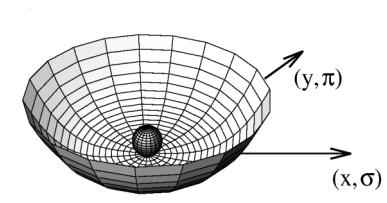
\includegraphics[width=0.49\textwidth]{images/higgs_mechanism.png}
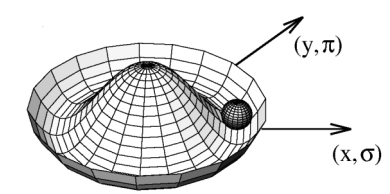
\includegraphics[width=0.49\textwidth]{images/higgs_mechanism_broken.png}
\end{center}
\begin{itemize}
\item
The Higgs field is the simplest of several proposed causes for electroweak symmetry breaking and the means by which elementary particles acquire mass.
\item
The Higgs boson is the smallest possible excitation of the Higgs field.
\end{itemize}
%\begin{itemize}
%\item
%  When you have spontaneous symmetry breaking you get Goldstone bosons.
%\item
%  Peter Higgs showed that when a local symmetry is spontaneously broken in a relativistic theory instead of Goldstone bosons you get a m%assive vector field.
%\item
%  The other mode is a massive spin-zero particle (Higgs boson).
%\end{itemize}
\end{frame}


%\begin{frame}{Higgs ``Description'' }
%\begin{center}
%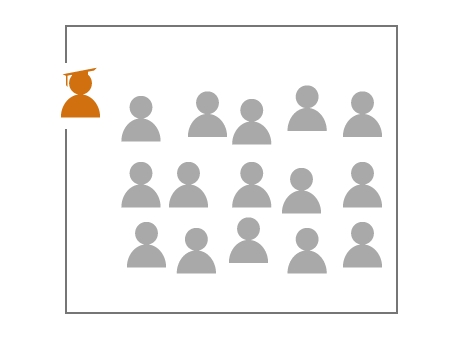
\includegraphics[width=0.89\textwidth]{images/higgs_cartoon-0.png}
%\end{center}
%\end{frame}

%\begin{frame}{Higgs ``Description'' }
%\begin{center}
%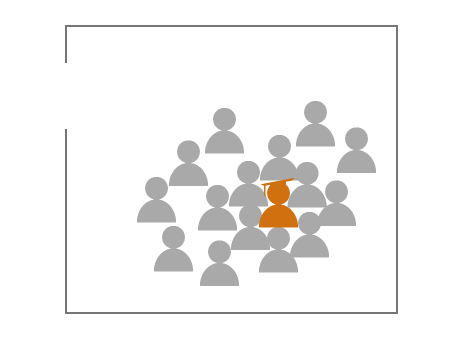
\includegraphics[width=0.89\textwidth]{images/higgs_cartoon-1.png}
%\end{center}
%\end{frame}

%\begin{frame}{Higgs ``Description'' }
%\begin{center}
%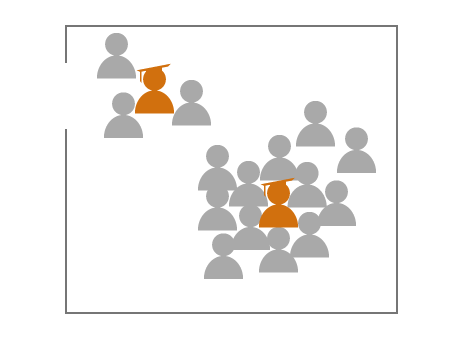
\includegraphics[width=0.89\textwidth]{images/higgs_cartoon-2.png}
%\end{center}
%\end{frame}

